Dans ce chapitre, nous décrirons les sources des données utilisées pour le calcul de la valeur moyenne de concentration de radon.

\section{Base de données nationale du radon}
La source principale des données est la BDD nationale du radon. Cette BDD contient 279'257 entrées, une pour chaque mesure de radon effectuée.
Elle a été exportée initialement sous forme de fichier excel nommé "Messungen\_020721.xlsx". C'est ce fichier que nous considèreront comme la source initiale des données. % TODO est-ce qu'on peut référencer ces données de façon plus précise?

\begin{itemize}
\item \textbf{Période de récolte des données} [1982]-[2021] % TODO est-ce que c'est correct?
\item \textbf{Date de publication} 2021-07-02
\item \textbf{Lien vers les données} Données non disponibles publiquement
\end{itemize}

\section{Nombre d'étages des bâtiments par canton}\label{sectionCantonEtagesBatiments}
Afin d'effectuer la correction mentionnée au point \ref{introCorrectionEtage} il est nécessaire d'avoir des données concernant l'étage d'habitation moyen par canton. Malheureusement, cette information n'est pas disponible directement sur le catalogue de données de l'OFS. Ce qui est par contre disponible, c'est le nombre de bâtiments qui ont un certain nombre d'étages, par canton. Pour obtenir le fichier source dans le format que le programme accepte, il faut aller sur ce lien \url{https://www.pxweb.bfs.admin.ch/pxweb/fr/px-x-0902010000_101/px-x-0902010000_101/px-x-0902010000_101.px} et sélectionner les options comme dans la figure \ref{fig:nbFloorsBuildingExportOptions}. Il faut ensuite cliquer sur le bouton "Continuer" et enregistrer les données sous forme de fichier CSV.

\begin{figure}[H]
    \centering
    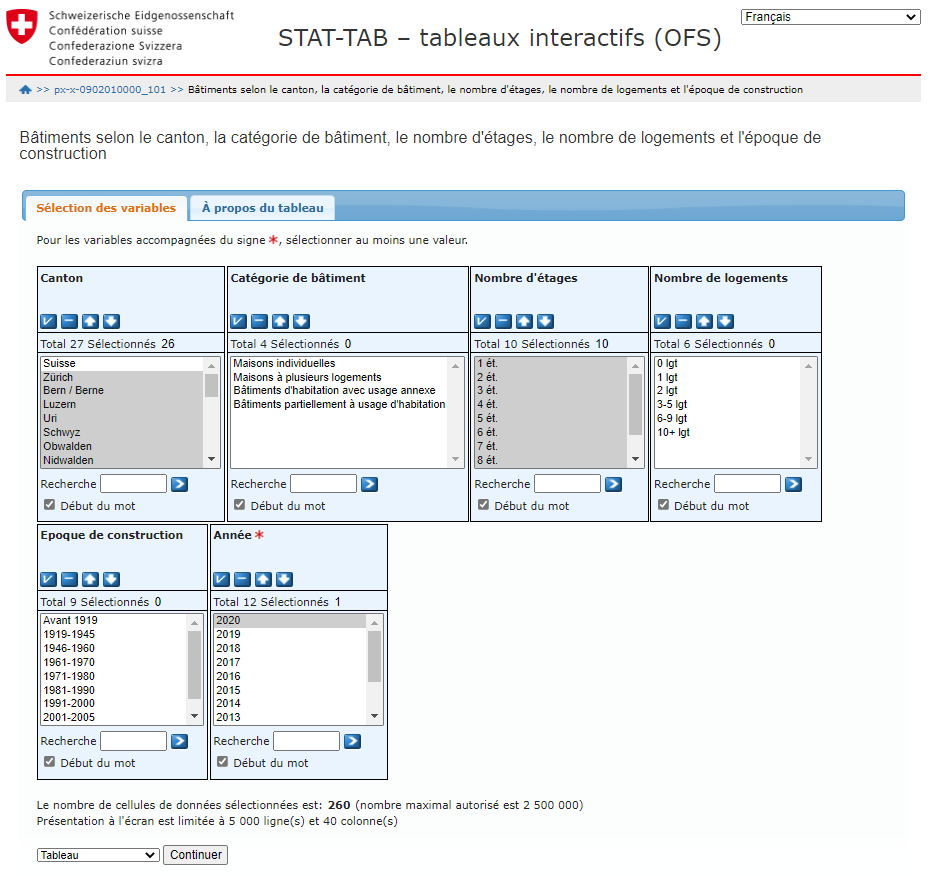
\includegraphics[width=\textwidth]{nb-floors-building-export-options}
    \caption{Options à sélectionner pour exporter les données du nombre d'étage des bâtiments par canton}
    \label{fig:nbFloorsBuildingExportOptions}
\end{figure}

Dans le chapitre \ref{chapterImportationEtPretraitement} nous expliquerons comment passer de ces données brutes à l'étage moyen d'habitation de la population, par canton.

\begin{itemize}
\item \textbf{Période de récolte des données} [2009]-[2020]
\item \textbf{Date de publication} 2021-10-07
\item \textbf{Lien vers les données} \url{https://www.bfs.admin.ch/bfs/fr/home/statistiques/construction-logement/batiments.assetdetail.19024696.html}
\end{itemize}


\section{Nombre d'habitants par commune}\label{sectionNombreHabitantsCommunes}
La moyenne de concentration est pondérée pour chaque commune par le nombre d'habitants dans la commune. Il est donc nécessaire d'avoir la population de chaque commune suisse. 

\begin{itemize}
\item \textbf{Période de récolte des données} [2004]-[2020]
\item \textbf{Date de publication} 2021-03-26
\item \textbf{Lien vers les données} \url{https://www.bfs.admin.ch/bfs/fr/home/statistiques/statistique-regions/portraits-regionaux-chiffres-cles/communes.assetdetail.15864461.html}
\end{itemize} 